\documentclass[12pt]{report}

\usepackage{geometry}
\usepackage{graphicx}
\usepackage{color}
\usepackage{listings}
\usepackage{xcolor}
\usepackage{hyperref}

% use double spacing
\usepackage{setspace}
\doublespacing

\geometry{a4paper}

\definecolor{ocre}{RGB}{243,102,25}
\definecolor{mygray}{RGB}{243,243,244}
\definecolor{deepGreen}{RGB}{26,111,0}
\definecolor{shallowGreen}{RGB}{235,255,255}
\definecolor{deepBlue}{RGB}{61,124,222}
\definecolor{shallowBlue}{RGB}{235,249,255}
\definecolor{codegreen}{rgb}{0,0.6,0.0}
\definecolor{codegray}{rgb}{0.5,0.5,0.5}
\definecolor{codepurple}{rgb}{0.58,0.2,0.82}
\definecolor{backcolour}{rgb}{0.95,0.95,0.92}
 
\lstdefinestyle{mystyle}{
    backgroundcolor=\color{backcolour},
    commentstyle=\color{codegreen},
    keywordstyle=\color{deepBlue},
    numberstyle=\tiny\color{codegray},
    stringstyle=\color{codepurple},
    basicstyle=\ttfamily\footnotesize,
    breakatwhitespace=false,         
    breaklines=true,                 
    captionpos=b,                    
    keepspaces=true,                 
    numbers=left,                    
    numbersep=5pt,                  
    showspaces=true,                
    showstringspaces=true,
    showtabs=true,                  
    tabsize=4
}
\lstset{style=mystyle}

\begin{document}
\begin{titlepage}
	\topskip0pt
	\vspace*{\fill}

	\begin{center}


		
\includegraphics[width=0.6\textwidth]{images/logo.png}

		\vspace{2cm}

		\Huge
		\textbf{Evolutionary Algorithms}
		\vspace{5.5cm}

		\Large

		\textbf{ \href{mailto:mq06861@st.habib.edu.pk}{Muhammad Meesum Ali Qazalbash - mq06861}}\\
		\textbf{ \href{mailto:@st.habib.edu.pk}{{Syed Ibrahim Ali Haider - sh06565}}}

		\vspace{0.5cm}

		\today

		CS451 - Computational Intelligence

		\vspace{0.5cm}
		\large
		Assignment 2
	\end{center}

	\vspace*{\fill}
\end{titlepage}

\setcounter{page}{2}
\tableofcontents

\chapter{Abstract}
The assignment focuses on swarm intelligence and provides students hands-on with Ant Colony Optimization (ACO) and Particle Swarm Optimization (PSO) techniques to solve complex optimization problems.

\chapter{Problems}

\section{Capacitated Vehicle Routing using ACO}

\subsection{External Modules}
There are three external modules used. Run the following command to download them.
\begin{lstlisting}[language=bash]
pip install numpy vrplib matplotlib
\end{lstlisting}

If this does not work then use,
\begin{lstlisting}[language=bash]
pip3 install numpy vrplib matplotlib
\end{lstlisting}

\lstinputlisting[language=python, caption= {External modules for ACO},linerange={1-3},firstnumber=1]{../CVRP/CVRP.py}

\subsection{Chromosome}
The class {\tt Ant\_t} is used to represent the chromosome. It contains routes and distance.
\lstinputlisting[language=python, caption= {Chromosome for ACO},linerange={6-17},firstnumber=6]{../CVRP/CVRP.py}

\newpage

\subsection{Initialization}
\lstinputlisting[language=python, caption= {Initilization of ACO},linerange={20-41},firstnumber=20]{../CVRP/CVRP.py}

\newpage

\subsection{Reading Input}
Note that the {\tt read\_file} does not depends on the object that's why it is a static method. This function would work when internet is avaible. If you get an error about the http request then make sure that you are connected to the internet.
\lstinputlisting[language=python, caption= {Reading input for ACO},linerange={43-70},firstnumber=43]{../CVRP/CVRP.py}

\subsection{Mathematics}
The mathematics for Ant Colony Optimization is implemented in the following functions.
\lstinputlisting[language=python, caption= {Mathematics for ACO},linerange={72-121},firstnumber=72]{../CVRP/CVRP.py}

\subsection{Simulation}
All the functions related to simulation are implemented in the following functions.
\lstinputlisting[language=python, caption= {Simulation for ACO},linerange={123-254},firstnumber=123]{../CVRP/CVRP.py}

\subsection{Plotting}
The plotting is done using the {\tt matplotlib} library. The following function is used to plot the results.
\lstinputlisting[language=python, caption= {Plotting for ACO},linerange={256-288},firstnumber=256]{../CVRP/CVRP.py}

\newpage

\subsection{Running}
The following piece of code is used to run the program.
\lstinputlisting[language=python, caption= {Running ACO},linerange={291-305},firstnumber=291]{../CVRP/CVRP.py}

\chapter{Analysis}
\section{Capacitated Vehicle Routing using ACO}

The analysis is done by varying the number of ants and the number of iterations. The results are shown in the following figures. In each grid number of ants are changing from 20 to 30 horizontally and number of iterations are changing from 20 to 30 vertically. Other parameters are \(\alpha = 4\), \(\beta = 4\), and \(\rho = 0.5\).

\begin{figure}[!ht]
	\centering
	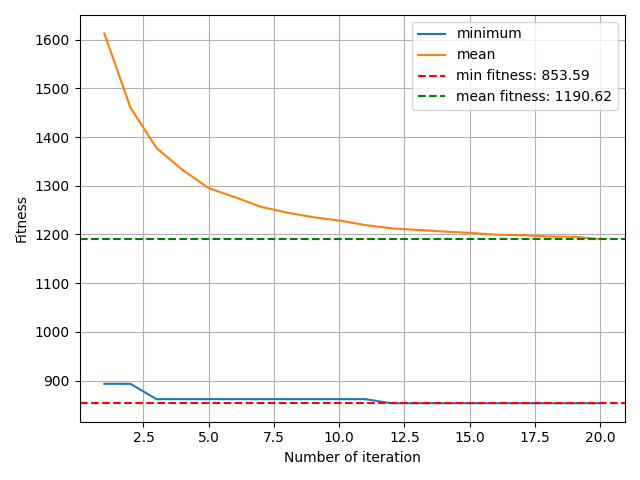
\includegraphics[width=0.4\textwidth]{../CVRP/plots/A-n32-k5-20-20.png}
	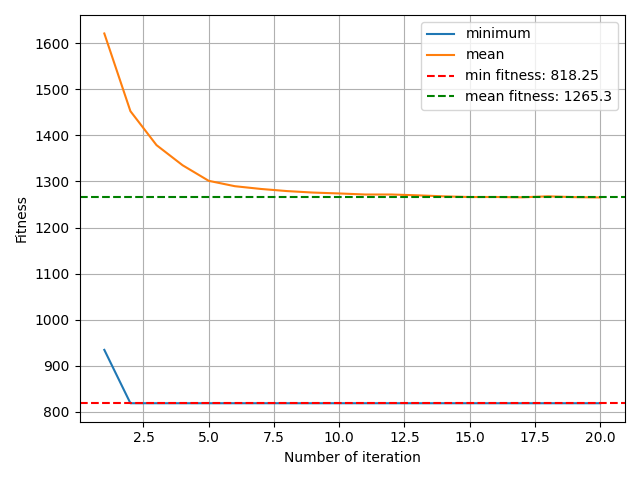
\includegraphics[width=0.4\textwidth]{../CVRP/plots/A-n32-k5-20-30.png}
	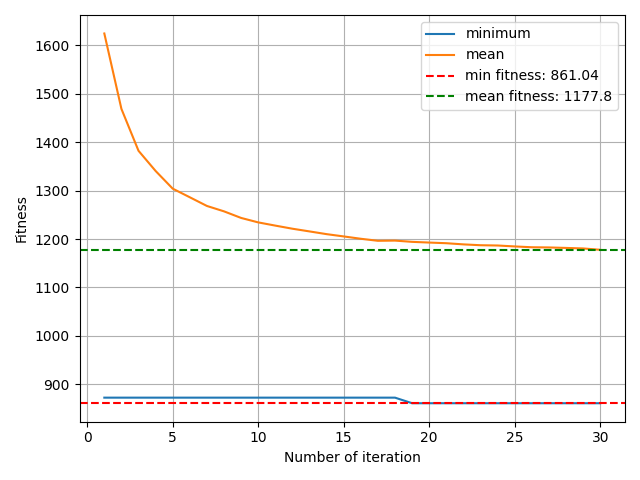
\includegraphics[width=0.4\textwidth]{../CVRP/plots/A-n32-k5-30-20.png}
	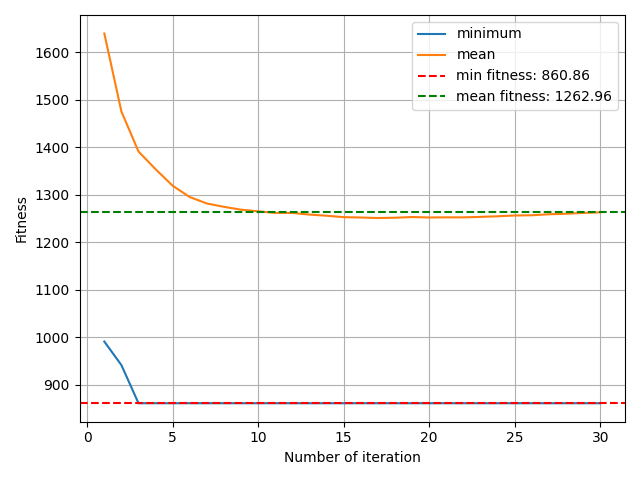
\includegraphics[width=0.4\textwidth]{../CVRP/plots/A-n32-k5-30-30.png}
	\caption{Dataset: A-n32-k5}
	\label{fig:A-n32-k5}
\end{figure}

%%%%

\begin{figure}[!ht]
	\centering
	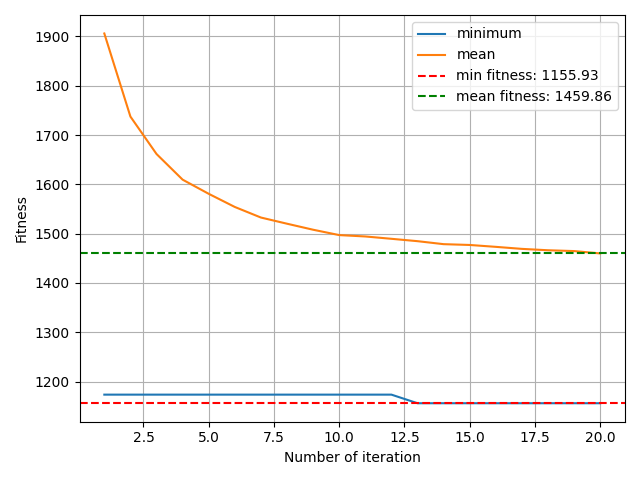
\includegraphics[width=0.4\textwidth]{../CVRP/plots/A-n44-k6-20-20.png}
	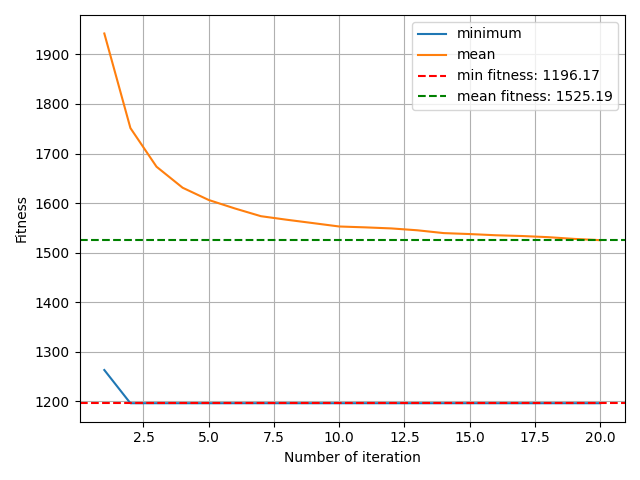
\includegraphics[width=0.4\textwidth]{../CVRP/plots/A-n44-k6-20-30.png}
	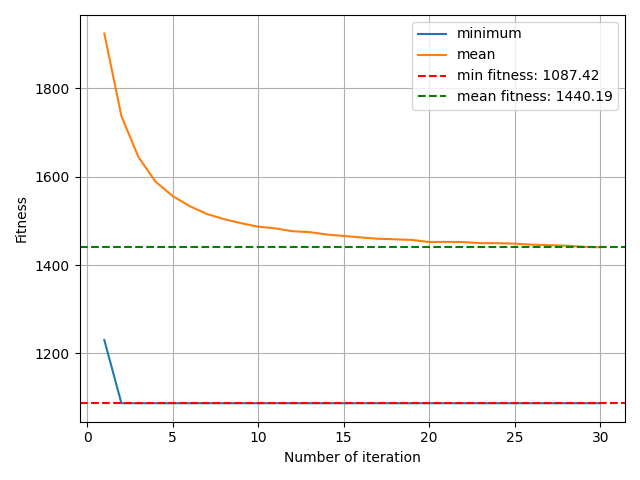
\includegraphics[width=0.4\textwidth]{../CVRP/plots/A-n44-k6-30-20.png}
	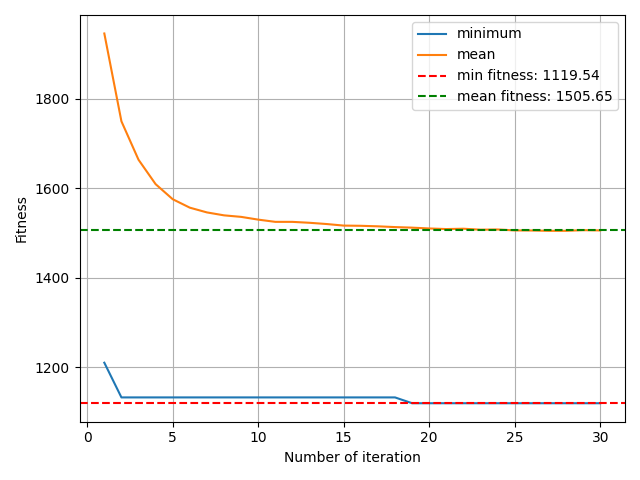
\includegraphics[width=0.4\textwidth]{../CVRP/plots/A-n44-k6-30-30.png}
	\caption{Dataset: A-n44-k6}
	\label{fig:A-n44-k6}
\end{figure}

%%%%

\begin{figure}[!ht]
	\centering
	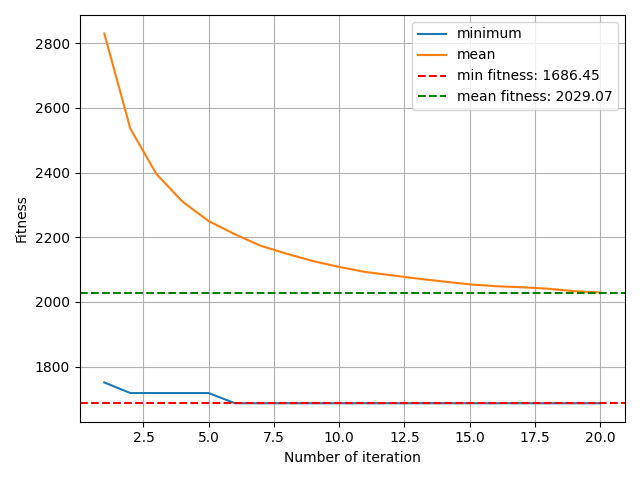
\includegraphics[width=0.4\textwidth]{../CVRP/plots/A-n60-k9-20-20.png}
	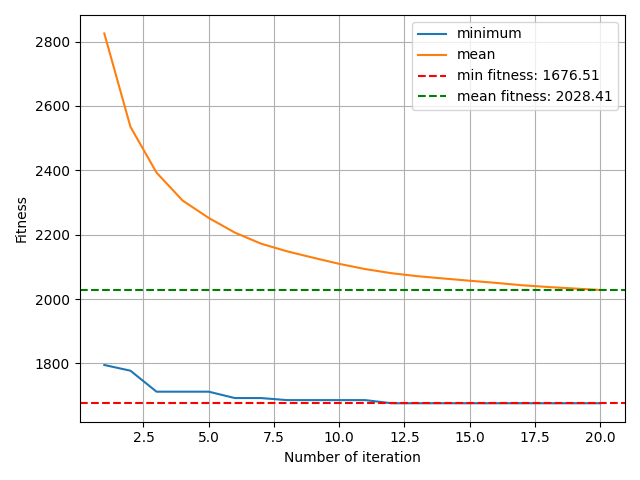
\includegraphics[width=0.4\textwidth]{../CVRP/plots/A-n60-k9-20-30.png}
	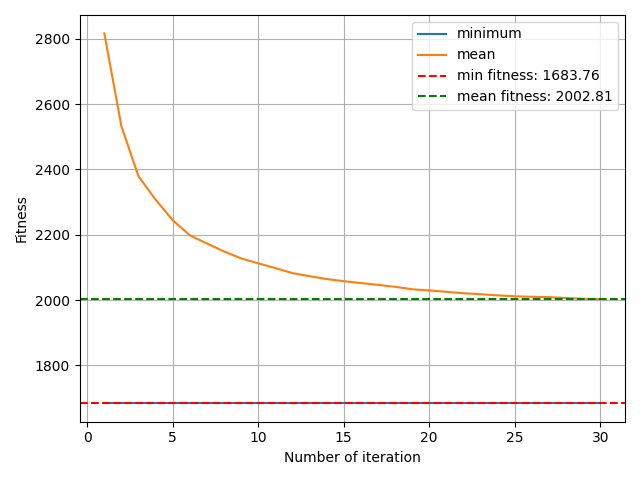
\includegraphics[width=0.4\textwidth]{../CVRP/plots/A-n60-k9-30-20.png}
	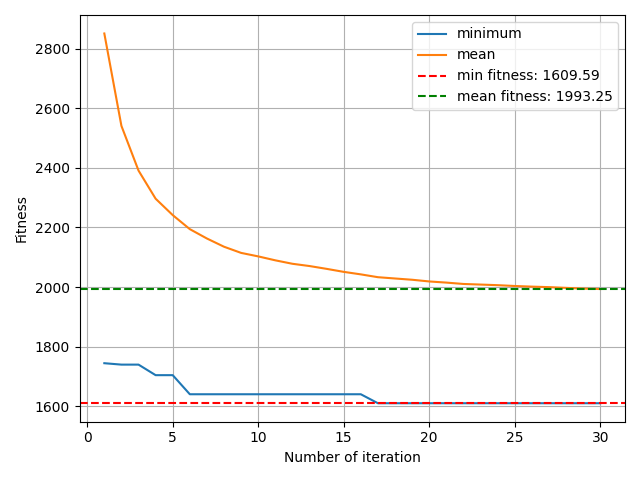
\includegraphics[width=0.4\textwidth]{../CVRP/plots/A-n60-k9-30-30.png}
	\caption{Dataset: A-n60-k9}
	\label{fig:A-n60-k9}
\end{figure}

%%%%

\begin{figure}[!ht]
	\centering
	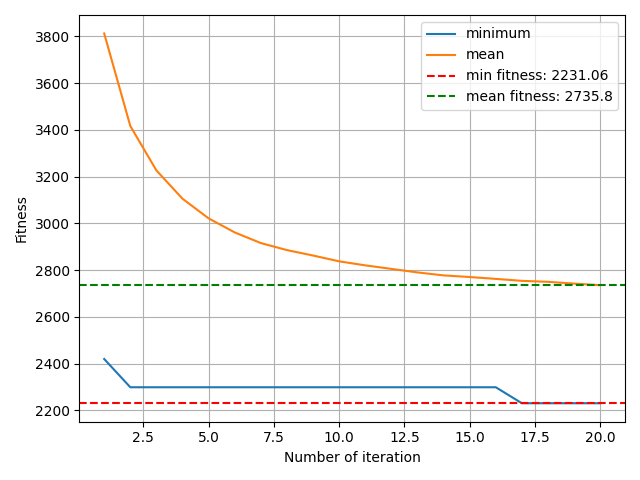
\includegraphics[width=0.4\textwidth]{../CVRP/plots/A-n80-k10-20-20.png}
	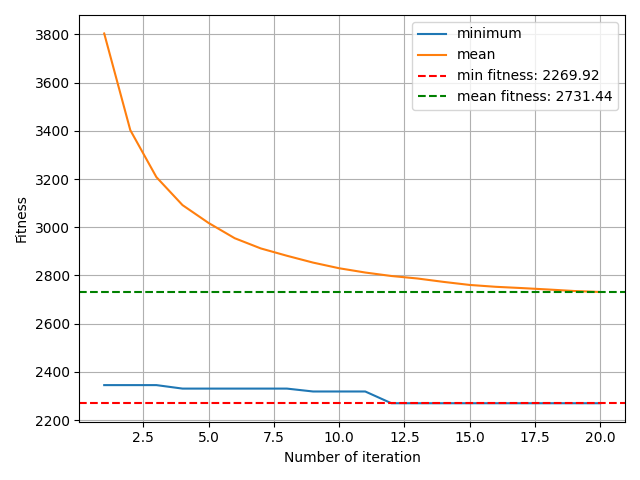
\includegraphics[width=0.4\textwidth]{../CVRP/plots/A-n80-k10-20-30.png}
	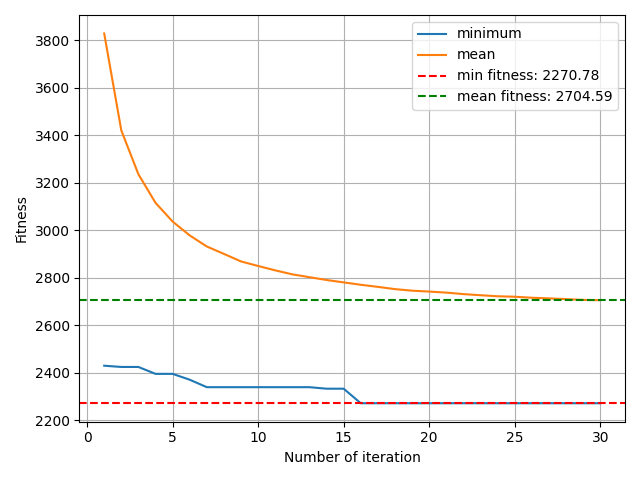
\includegraphics[width=0.4\textwidth]{../CVRP/plots/A-n80-k10-30-20.png}
	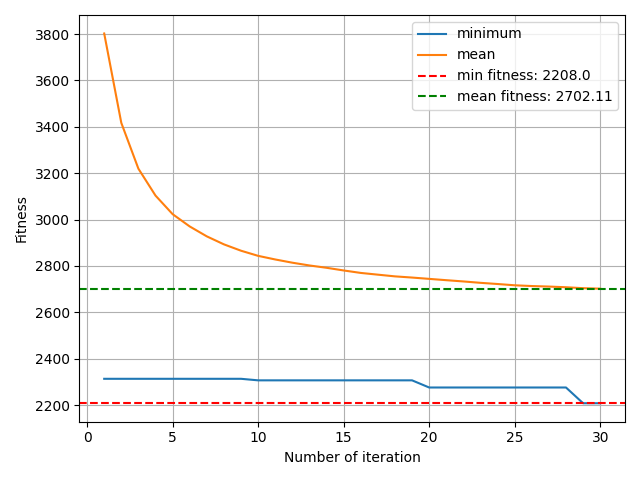
\includegraphics[width=0.4\textwidth]{../CVRP/plots/A-n80-k10-30-30.png}
	\caption{Dataset: A-n80-k10}
	\label{fig:A-n80-k10}
\end{figure}

\end{document}